به طور کلی در این مسئله ما 
\(2 * 5 = 10\) 
حالت داریم که آن‌ها را با زوج مرتب نشان می‌دهیم. عضو اول نشان‌دهنده جایگاه و عضو دوم نشان‌‌دهنده قطبیت در آن حالت است.

\[
\Sigma = \{ 1,2 \}
\]
\[
Q = \{ (s,p) \ | \ s \in \{0,1,2,3,4\} \ , \ p\in\{+,-\} \}
\]
حالت شروع و پایان:
\[
q_0 = (0,+) \ \ \ \ q_F = (0,+)\]

تابع انتقال:

\begin{table}[h]
    \centering
    \begin{RTL}
    \begin{tabular}{|c|c|c|}
    \hline
    2 & 1 & state \\
    \hline
    $(2,-)$ & $(1,+)$ & $(0,+)$ \\
    $(3,-)$ & $(4,-)$ & $(0,-)$ \\
    $(3,+)$ & $(2,-)$ & $(1,+)$ \\
    $(4,-)$ & $(0,-)$ & $(1,-)$ \\
    $(4,+)$ & $(3,+)$ & $(2,+)$ \\
    $(0,-)$ & $(1,-)$ & $(2,-)$ \\
    $(0,+)$ & $(4,+)$ & $(3,+)$ \\
    $(1,-)$ & $(2,+)$ & $(3,-)$ \\
    $(1,+)$ & $(0,+)$ & $(4,+)$ \\
    $(2,+)$ & $(3,-)$ & $(4,-)$ \\
    \hline
    \end{tabular}
    \end{RTL}
    \end{table}

نمودار \lr{DFA}:


\begin{center}
    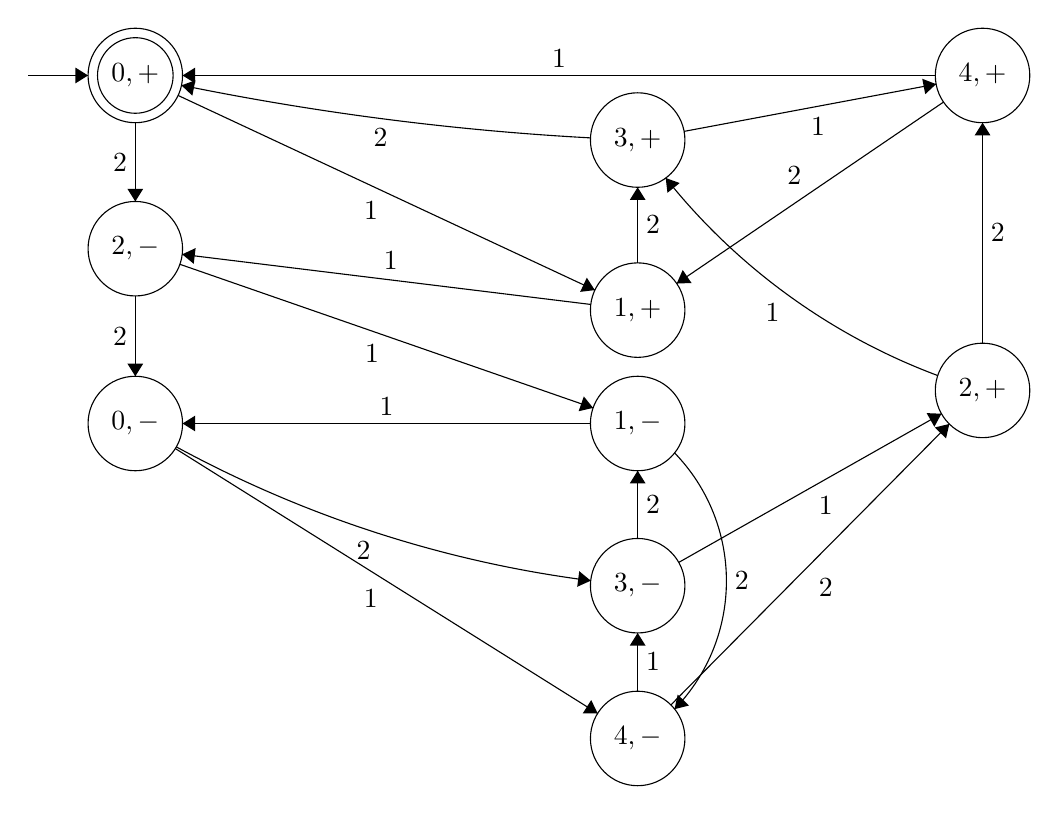
\begin{tikzpicture}[scale=0.2]
    \tikzstyle{every node}+=[inner sep=0pt]
    \draw [black] (7.7,-4.3) circle (3);
    \draw (7.7,-4.3) node {$0,+$};
    \draw [black] (7.7,-4.3) circle (2.4);
    \draw [black] (39.6,-19.2) circle (3);
    \draw (39.6,-19.2) node {$1,+$};
    \draw [black] (7.7,-26.4) circle (3);
    \draw (7.7,-26.4) node {$0,-$};
    \draw [black] (39.6,-26.4) circle (3);
    \draw (39.6,-26.4) node {$1,-$};
    \draw [black] (7.7,-15.3) circle (3);
    \draw (7.7,-15.3) node {$2,-$};
    \draw [black] (39.6,-36.7) circle (3);
    \draw (39.6,-36.7) node {$3,-$};
    \draw [black] (39.6,-46.4) circle (3);
    \draw (39.6,-46.4) node {$4,-$};
    \draw [black] (61.5,-24.3) circle (3);
    \draw (61.5,-24.3) node {$2,+$};
    \draw [black] (39.6,-8.4) circle (3);
    \draw (39.6,-8.4) node {$3,+$};
    \draw [black] (61.5,-4.3) circle (3);
    \draw (61.5,-4.3) node {$4,+$};
    \draw [black] (10.42,-5.57) -- (36.88,-17.93);
    \fill [black] (36.88,-17.93) -- (36.37,-17.14) -- (35.95,-18.04);
    \draw (22.67,-12.26) node [below] {$1$};
    \draw [black] (7.7,-7.3) -- (7.7,-12.3);
    \fill [black] (7.7,-12.3) -- (8.2,-11.5) -- (7.2,-11.5);
    \draw (7.2,-9.8) node [left] {$2$};
    \draw [black] (10.24,-27.99) -- (37.06,-44.81);
    \fill [black] (37.06,-44.81) -- (36.65,-43.96) -- (36.11,-44.81);
    \draw (22.65,-36.9) node [below] {$1$};
    \draw [black] (36.617,-36.38) arc (-97.27003:-118.51885:74.98);
    \fill [black] (36.62,-36.38) -- (35.89,-35.78) -- (35.76,-36.77);
    \draw (22.19,-33.9) node [below] {$2$};
    \draw [black] (36.62,-18.84) -- (10.68,-15.66);
    \fill [black] (10.68,-15.66) -- (11.41,-16.26) -- (11.53,-15.26);
    \draw (23.92,-16.66) node [above] {$1$};
    \draw [black] (39.6,-16.2) -- (39.6,-11.4);
    \fill [black] (39.6,-11.4) -- (39.1,-12.2) -- (40.1,-12.2);
    \draw (40.1,-13.8) node [right] {$2$};
    \draw [black] (36.6,-26.4) -- (10.7,-26.4);
    \fill [black] (10.7,-26.4) -- (11.5,-26.9) -- (11.5,-25.9);
    \draw (23.65,-25.9) node [above] {$1$};
    \draw [black] (41.94,-28.264) arc (44.10959:-44.10959:11.689);
    \fill [black] (41.94,-44.54) -- (42.86,-44.31) -- (42.14,-43.61);
    \draw (45.74,-36.4) node [right] {$2$};
    \draw [black] (58.653,-23.355) arc (-110.51095:-141.4504:40.014);
    \fill [black] (41.38,-10.81) -- (41.49,-11.75) -- (42.27,-11.13);
    \draw (48.16,-18.76) node [below] {$1$};
    \draw [black] (61.5,-21.3) -- (61.5,-7.3);
    \fill [black] (61.5,-7.3) -- (61,-8.1) -- (62,-8.1);
    \draw (62,-14.3) node [right] {$2$};
    \draw [black] (10.53,-16.29) -- (36.77,-25.41);
    \fill [black] (36.77,-25.41) -- (36.18,-24.68) -- (35.85,-25.62);
    \draw (22.74,-21.38) node [below] {$1$};
    \draw [black] (7.7,-18.3) -- (7.7,-23.4);
    \fill [black] (7.7,-23.4) -- (8.2,-22.6) -- (7.2,-22.6);
    \draw (7.2,-20.85) node [left] {$2$};
    \draw [black] (42.55,-7.85) -- (58.55,-4.85);
    \fill [black] (58.55,-4.85) -- (57.67,-4.51) -- (57.86,-5.49);
    \draw (51.06,-6.94) node [below] {$1$};
    \draw [black] (36.603,-8.263) arc (-93.10063:-101.54713:177.768);
    \fill [black] (10.63,-4.93) -- (11.32,-5.58) -- (11.52,-4.6);
    \draw (23.27,-7.66) node [below] {$2$};
    \draw [black] (42.21,-35.22) -- (58.89,-25.78);
    \fill [black] (58.89,-25.78) -- (57.95,-25.74) -- (58.44,-26.61);
    \draw (51.55,-31) node [below] {$1$};
    \draw [black] (39.6,-33.7) -- (39.6,-29.4);
    \fill [black] (39.6,-29.4) -- (39.1,-30.2) -- (40.1,-30.2);
    \draw (40.1,-31.55) node [right] {$2$};
    \draw [black] (58.5,-4.3) -- (10.7,-4.3);
    \fill [black] (10.7,-4.3) -- (11.5,-4.8) -- (11.5,-3.8);
    \draw (34.6,-3.8) node [above] {$1$};
    \draw [black] (59.02,-5.99) -- (42.08,-17.51);
    \fill [black] (42.08,-17.51) -- (43.02,-17.48) -- (42.46,-16.65);
    \draw (49.55,-11.25) node [above] {$2$};
    \draw [black] (39.6,-43.4) -- (39.6,-39.7);
    \fill [black] (39.6,-39.7) -- (39.1,-40.5) -- (40.1,-40.5);
    \draw (40.1,-41.55) node [right] {$1$};
    \draw [black] (41.71,-44.27) -- (59.39,-26.43);
    \fill [black] (59.39,-26.43) -- (58.47,-26.65) -- (59.18,-27.35);
    \draw (51.07,-36.83) node [right] {$2$};
    \draw [black] (0.9,-4.3) -- (4.7,-4.3);
    \fill [black] (4.7,-4.3) -- (3.9,-3.8) -- (3.9,-4.8);
    \end{tikzpicture}
    \end{center}
    